% =====================================================================
% THIS FILE IS THE SOURCE. Edit it, then rebuild the PDF with:
%     bash tools/compile.sh Unit_13_Choosing_a_Model
% (run from the Alternative_Model_First folder; it compiles twice and
%  reports page count, overfull boxes, and em dashes)
%
% OPTIONAL UNIT. It is not part of the 12-unit calendar. It sits most
% naturally after Unit 4 (Prediction), and it deliberately forward-
% references logistic regression (Unit 11) and count models (Units 7-8)
% rather than teaching them.
%
% Figures: fig_u13_*.pdf, regenerated by tools/make_unit13_slide_figs.py
% Do not edit the PDF directly.
% =====================================================================
\documentclass[aspectratio=169]{beamer}
\usetheme{default}
\usefonttheme{professionalfonts}
\usepackage{amsmath, amssymb, amsfonts}
\usepackage{graphicx}
\usepackage{booktabs}
\usepackage{bm}
\usepackage{hyperref}

\mode<presentation> {
    \usetheme{Frankfurt}
    \usecolortheme{default}
}

% == notation shortcuts ==
\newcommand{\xbar}{\bar{x}}
\newcommand{\yhat}{\hat{y}}

% Recurring motifs (color-coded).
\newenvironment{principle}[1]{\begin{block}{\textbf{Principle:} #1}}{\end{block}}
\newenvironment{trap}[1]{\begin{alertblock}{\textbf{Trap:} #1}}{\end{alertblock}}
\newenvironment{practice}[1]{\begin{exampleblock}{\textbf{In practice:} #1}}{\end{exampleblock}}
\newenvironment{interview}[1]{\begin{exampleblock}{\textbf{You may be asked:} #1}}{\end{exampleblock}}
\newenvironment{yourturn}[1]{%
  \setbeamercolor{block title}{fg=white,bg=orange!80!black}%
  \setbeamercolor{block body}{bg=orange!12}%
  \begin{block}{\textbf{Your turn:} #1}}{\end{block}}
\newenvironment{livedemo}[1]{%
  \setbeamercolor{block title}{fg=white,bg=teal!80!black}%
  \setbeamercolor{block body}{bg=teal!12}%
  \begin{block}{\textbf{Live demo:} #1}}{\end{block}}
\newenvironment{llmcheck}[1]{%
  \setbeamercolor{block title}{fg=white,bg=violet!75!black}%
  \setbeamercolor{block body}{bg=violet!10}%
  \begin{block}{\textbf{LLM check:} #1}}{\end{block}}

\title{Choosing a Model}
\subtitle{Unit 13 (optional): When a More Complicated Model Earns Its Keep}
\author{Stat 220 \textbar{} Statistics for Data Science}
\date{}

\begin{document}

\begin{frame}
  \titlepage
\end{frame}

% ======================================================================
\section{Why}
% ======================================================================
\begin{frame}{Where we left off}
\begin{itemize}
  \item Unit 2 read a slope. Unit 3 built models with many predictors and judged them honestly.
        Unit 4 put error bars on a single prediction.
  \item Every one of those units assumed somebody had already handed you the model.
  \item Nobody ever said how that choice gets made.
\end{itemize}
\begin{principle}{the gap this unit fills}
You know how to fit a model and how to check whether it is any good. This unit is about the step
before both of those: deciding which model to reach for, and being able to say why.
\end{principle}
\end{frame}

\begin{frame}{The question nobody answered for you}
\begin{itemize}
  \item ``Should I use linear regression or a random forest?'' is the most common real question in
        applied work, and the least often taught.
  \item The honest answer is never ``the fancy one'' and never ``the simple one.'' It depends on
        four things you can actually check: your question, your outcome, your sample size, and
        what it costs you to be wrong.
  \item This unit turns that into something you can do out loud, in order, in an interview or a
        meeting.
\end{itemize}
\begin{practice}{the shape of this unit}
``We have 300 rows, 40 candidate predictors, and we need to know whether the price change hurt
retention. What would you fit?''
\end{practice}
\end{frame}

\begin{frame}{What this unit gives you}
\begin{columns}[T]
\begin{column}{0.5\textwidth}
\textbf{Things to know}
\begin{itemize}\small
  \item the four questions a model can be asked, and that they are separate
  \item bias and variance as the reason the error curve is U-shaped
  \item what actually moves the best complexity: $n$, noise, and the number of candidates
  \item which model families answer which question well
  \item what each family costs you in interpretability and in data
\end{itemize}
\end{column}
\begin{column}{0.5\textwidth}
\textbf{Mistakes to stop making}
\begin{itemize}\small
  \item reaching for a flexible model on 40 rows
  \item reaching for a simple model on 400{,}000 and calling it caution
  \item using a prediction model's coefficients as effects
  \item choosing the model after seeing which one gave the answer you wanted
  \item reporting the winner of a long search as if it were the only thing you tried
\end{itemize}
\end{column}
\end{columns}
\end{frame}

% ======================================================================
\section{Four questions}
% ======================================================================
\begin{frame}{The four questions a model gets asked}
\begin{enumerate}
  \item \textbf{Is $X$ important?} One variable, one verdict.
  \item \textbf{Which variables are important?} A list, out of many candidates.
  \item \textbf{What is the predicted value?} A number for a new case.
  \item \textbf{How certain am I?} An honest range around any of the above.
\end{enumerate}
\vspace{0.3em}
\begin{principle}{they are not the same question}
These four look like one job because a single \texttt{fit()} call seems to answer all of them at
once. It does not. A model can be excellent at question 3 and actively misleading on question 1.
\end{principle}
\end{frame}

\begin{frame}{One model, four different grades}
\small
Same 392 cars, same random forest predicting mpg.
\begin{center}\footnotesize
\begin{tabular}{p{0.30\textwidth} p{0.16\textwidth} p{0.44\textwidth}}
\toprule
\textbf{Question} & \textbf{Grade} & \textbf{Why} \\
\midrule
Is weight important? & poor & Importance scores split credit among correlated predictors. Weight and displacement steal from each other. \\
Which variables matter? & fair & It ranks them, but the ranking shifts every refit and says nothing about direction. \\
What is the predicted mpg? & strong & This is what the model optimizes. \\
How certain am I? & fair & You can get an interval from held-out errors, but not from the model itself. \\
\bottomrule
\end{tabular}
\end{center}
\begin{principle}{pick the tool for the question you were actually asked}
The forest is not a bad model. It is a bad answer to question 1.
\end{principle}
\end{frame}

\begin{frame}{Your turn \#1}
\begin{yourturn}{four teams, four questions}
A hospital has 5 years of records on 90{,}000 patients and 200 variables. Four people walk in with
four requests.
\begin{enumerate}\small
  \item Legal: ``Does our new intake form change how long patients wait?''
  \item Ops: ``Which 10 of these 200 things should we even be tracking?''
  \item The app team: ``Given a patient at check-in, how long will they wait?''
  \item The director: ``How sure are you about any of this?''
\end{enumerate}
\end{yourturn}
For each one, say what you would fit. Two of these want the same model family for very different
reasons. One of them is not a modeling question at all until you ask something first.
\end{frame}

\begin{frame}{Your turn \#1: answer}
\small
\begin{enumerate}
  \item \textbf{Legal wants one coefficient defended.} Regression with the intake form as the
        predictor of interest and the known confounders included on purpose. You need a slope
        with a standard error, not the best prediction. And ask first whether the form was rolled
        out in a way that lets you claim anything causal (Unit 5).
  \item \textbf{Ops wants a short list from 200 candidates.} Regularization, the lasso, which
        shrinks most coefficients to zero and keeps a handful. Report it as a screening list, not
        as ``these 10 cause wait times.''
  \item \textbf{The app wants a number.} Anything that predicts well. With 90{,}000 rows you can
        afford a forest or boosting, and nobody needs to read its coefficients.
  \item \textbf{The director wants uncertainty.} Not a model at all. Ask which of the first three
        she means, because the honest interval is different for each one.
\end{enumerate}
\begin{principle}{}
Questions 1 and 2 both use regression, and for opposite reasons: one defends a single coefficient,
the other throws most of them away.
\end{principle}
\end{frame}

% ======================================================================
\section{Complexity}
% ======================================================================
\begin{frame}{Simple or complicated, the honest version}
\begin{itemize}
  \item The question is not ``which model is better.'' Asked that way it has no answer.
  \item The question is: \textbf{do I have enough data to afford this much flexibility?}
  \item Flexibility is something you buy. The price is paid in sample size, and if you cannot
        afford it you do not get a slightly worse model, you get a much worse one.
\end{itemize}
\begin{principle}{the reframe}
A complicated model is not a stronger claim about the world. It is a bigger bet that you have
enough data to pin down what you just allowed to vary.
\end{principle}
\end{frame}

\begin{frame}{Two ways to be wrong}
\begin{columns}[T]
\begin{column}{0.48\textwidth}
\textbf{Too simple}
\begin{itemize}\small
  \item Wrong in the same direction every time.
  \item Fit it on fresh data and you get almost the same wrong answer.
  \item Stable, and stably off.
\end{itemize}
\centering\small (\textbf{bias})
\end{column}
\begin{column}{0.48\textwidth}
\textbf{Too complicated}
\begin{itemize}\small
  \item Right on average across many refits.
  \item But any single fit chases the noise in the rows you happened to draw.
  \item Refit on new data and it looks like a different model.
\end{itemize}
\centering\small (\textbf{variance})
\end{column}
\end{columns}
\vspace{0.4em}
\begin{principle}{why the error curve is U-shaped}
Adding flexibility trades one for the other. Bias falls, variance rises, and the total is worst at
both ends. The whole art is finding where the trade stops paying.
\end{principle}
\end{frame}

\begin{frame}{The U-shape, taken apart}
\begin{columns}[c]
\begin{column}{0.58\textwidth}
\centering
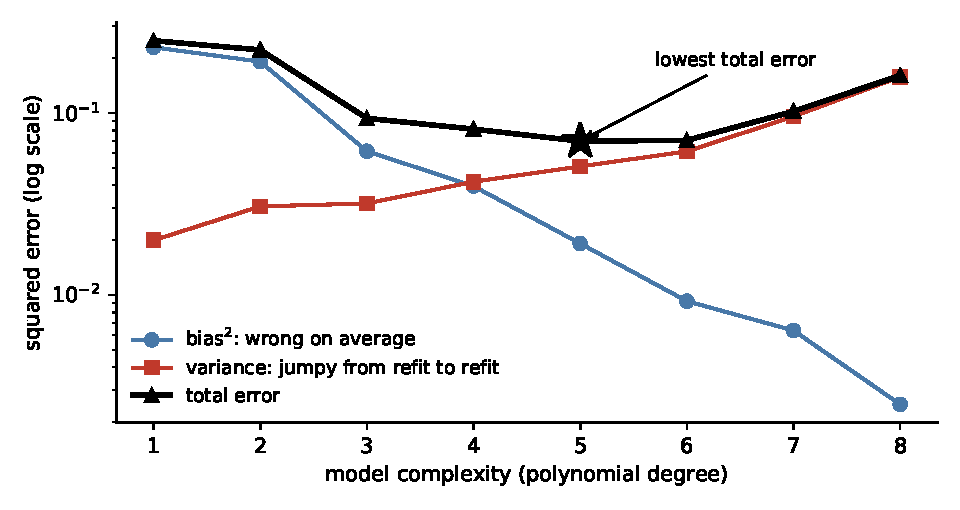
\includegraphics[width=\textwidth]{fig_u13_bias_variance.pdf}
\end{column}
\begin{column}{0.42\textwidth}
\small
600 datasets of $n = 60$, each fit with polynomials of every degree, compared against the true
curve we simulated.
\begin{itemize}
  \item Bias falls the whole way. More flexibility really does get closer to the truth on average.
  \item Variance climbs the whole way.
  \item Their sum bottoms out at degree 5.
\end{itemize}
\end{column}
\end{columns}
\onslide<2->{\centering\small
Neither curve has a minimum. Only the sum does.}
\end{frame}

\begin{frame}{Can you afford the truth?}
\begin{columns}[c]
\begin{column}{0.58\textwidth}
\centering
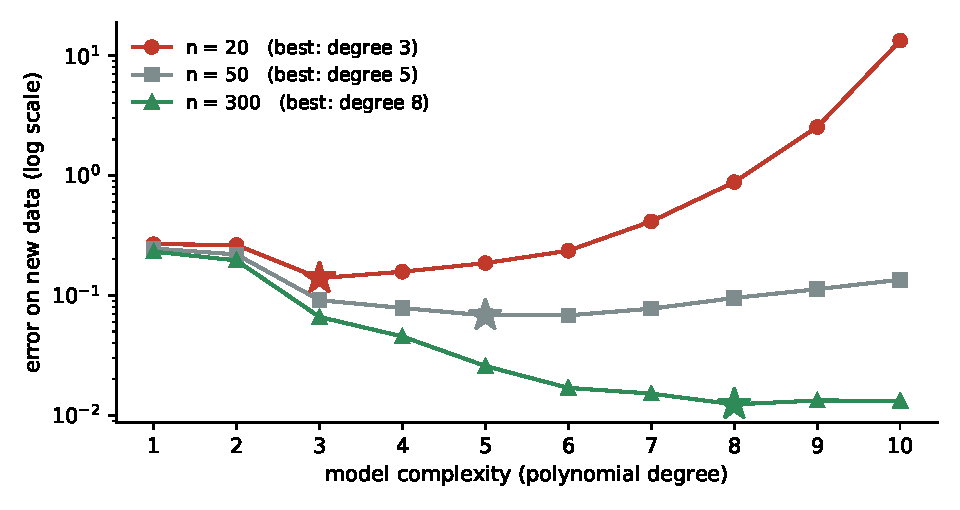
\includegraphics[width=\textwidth]{fig_u13_afford_truth.pdf}
\end{column}
\begin{column}{0.42\textwidth}
\small
The true curve never changes. The only thing that changes is how many rows you were given.
\begin{itemize}
  \item $n = 20$: best is degree \textbf{3}.
  \item $n = 50$: best is degree \textbf{5}.
  \item $n = 300$: best is degree \textbf{8}.
\end{itemize}
\end{column}
\end{columns}
\onslide<2->{\vspace{0.2em}\centering\small
Overshooting to degree 10 costs you a factor of \textbf{96} at $n = 20$, and \textbf{7 percent}
at $n = 300$. Same mistake, same model, opposite verdict.}
\end{frame}

\begin{frame}{What moves the best complexity}
\begin{center}\footnotesize
\begin{tabular}{p{0.34\textwidth} p{0.18\textwidth} p{0.36\textwidth}}
\toprule
\textbf{When this goes up} & \textbf{Best model gets} & \textbf{Because} \\
\midrule
Sample size $n$ & more complex & variance is the part data buys down \\
Noise in the outcome & simpler & more of what you would fit is noise \\
Candidate predictors $p$ & simpler & searching is itself a form of fitting \\
Smoothness of the truth & simpler & there is less structure to find \\
Cost of a confident error & simpler & stable models fail less spectacularly \\
Need to explain a coefficient & simpler & you cannot defend what you cannot read \\
\bottomrule
\end{tabular}
\end{center}
\begin{principle}{the one-line version}
More rows push you toward flexibility. Noise, candidates, and the need to explain push you back.
\end{principle}
\end{frame}

\begin{frame}{The same question, on real cars}
\begin{columns}[c]
\begin{column}{0.56\textwidth}
\centering
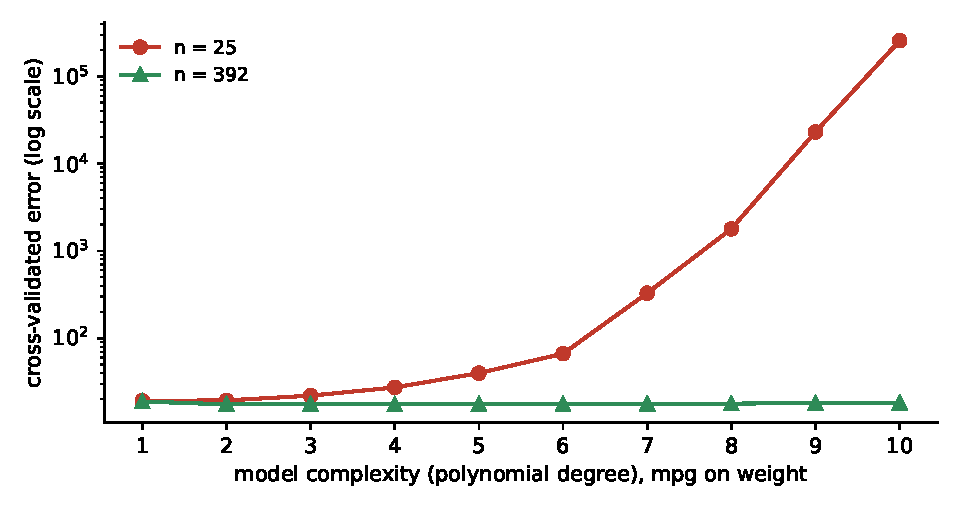
\includegraphics[width=\textwidth]{fig_u13_overshoot.pdf}
\end{column}
\begin{column}{0.44\textwidth}
\small
mpg on weight, cross-validated, real data.
\begin{itemize}
  \item The best degree hardly moves. The relationship really is close to a simple curve.
  \item What collapses is the \textbf{penalty for guessing too high}.
  \item At $n = 25$, overshooting to degree 10 is a catastrophe. At $n = 392$ it is nearly free.
\end{itemize}
\end{column}
\end{columns}
\onslide<2->{\centering\small
With enough data you are allowed to be wrong about complexity. With 25 rows you are not.}
\end{frame}

\begin{frame}{Your turn \#2}
\begin{yourturn}{same model, two companies}
Two teams both want to predict whether a customer churns next month. Both propose the identical
gradient-boosted model with 500 trees.
\begin{itemize}\small
  \item Team A works at a bank with 2.4 million customers and 60 clean variables.
  \item Team B works at a startup with 340 customers and 60 variables, most of them hand-entered.
\end{itemize}
\end{yourturn}
Same model, same code, same question. Is one of them making a mistake? Say which, and say what
they should do instead. Then say what would have to change for your answer to flip.
\end{frame}

\begin{frame}{Your turn \#2: answer}
\small
\begin{itemize}
  \item \textbf{Team A is fine.} With 2.4 million rows the variance cost of 500 trees is tiny, and
        that is exactly the regime where flexibility is cheap. They should still hold out a test
        set and still refuse to read the importances as effects.
  \item \textbf{Team B is not.} 340 rows and 60 hand-entered variables is the worst corner of the
        table: small $n$, large $p$, high noise. A boosted forest there will fit the data
        beautifully and predict new customers badly.
  \item \textbf{What B should do:} a regularized logistic regression on a handful of variables
        chosen for a reason, cross-validated, with the one-standard-error rule to break ties
        toward the simpler fit.
  \item \textbf{What would flip it:} B getting to a few tens of thousands of clean rows. Not a
        better algorithm. More data.
\end{itemize}
\begin{principle}{}
The model was never the problem. The ratio of what you are estimating to what you were given is.
\end{principle}
\end{frame}

% ======================================================================
\section{Activity}
% ======================================================================
\begin{frame}{Commit before you see the test set}
\begin{livedemo}{the whole unit in ten minutes}
On screen: 14 points, one predictor, one outcome. That is all anyone gets to look at.
\begin{enumerate}\small
  \item Each team writes a polynomial degree from 1 to 10 on a card and holds it up. Committed,
        before anything else happens.
  \item I fit every chosen degree live. Each team's curve goes on the plot. The high-degree curves
        visibly pass closer to the points, and teams that chose 8 or 9 feel good about it.
  \item I show the training error. The teams that chose high degrees are winning by a lot.
  \item Then I reveal the 10 held-out points that were there the whole time, and rescore.
\end{enumerate}
\end{livedemo}
Write the two leaderboards side by side on the board before revealing the second one.
\end{frame}

\begin{frame}{What happens every time we run this}
\begin{itemize}
  \item The training leaderboard is almost perfectly ordered by degree. Highest degree wins.
  \item The test leaderboard is close to reversed at the top, and the winner is usually a team
        that picked 2, 3, or 4.
  \item Nobody who picked 9 is anywhere near the top, and their curve is the one that looked best
        ten minutes ago.
\end{itemize}
\begin{principle}{the point of committing first}
You had to choose without seeing the test data. That is the real situation, always. Cross-validation
is how you make that choice honestly, using only the data you were allowed to look at.
\end{principle}
\begin{interview}{}
``How did you pick the complexity?'' has exactly one good answer, and it is not ``it fit best.''
\end{interview}
\end{frame}

% ======================================================================
\section{The catalog}
% ======================================================================
\begin{frame}{How to read a model catalog}
Ask three things, in this order. The first two narrow it to a family. The third picks within it.
\begin{enumerate}
  \item \textbf{What kind of outcome is it?} A number, a yes/no, a count, a category, a time
        until something happens. This is not negotiable and it eliminates most of the catalog.
  \item \textbf{Which of the four questions am I answering?} Explaining one effect, screening many,
        predicting, or quantifying uncertainty.
  \item \textbf{How much data do I have relative to what I am estimating?} This sets how much
        flexibility you can afford.
\end{enumerate}
\begin{trap}{the usual order}
Most people start at step 3 with ``what is the strongest algorithm,'' which is the only one of the
three that cannot be answered on its own.
\end{trap}
\end{frame}

\begin{frame}{When the outcome is a number}
\begin{center}\small
\begin{tabular}{p{0.26\textwidth} p{0.30\textwidth} p{0.34\textwidth}}
\toprule
\textbf{Reach for} & \textbf{When} & \textbf{What it costs you} \\
\midrule
Linear regression & you must defend a coefficient & assumes the shape is roughly a line \\
Regression with transforms or interactions & the shape bends, and you can say how & you have to specify the bend yourself \\
Lasso or ridge & many candidates, prediction focus & coefficients are shrunk, so no clean effects \\
A single tree & you want a rule someone can follow & unstable, and coarse at the edges \\
Forest or boosting & prediction is all that matters & no readable coefficients, needs a lot of rows \\
\bottomrule
\end{tabular}
\end{center}
\begin{principle}{}
Going down this table buys flexibility and spends interpretability. There is no row that gives you
both.
\end{principle}
\end{frame}

\begin{frame}{When the outcome is not a number}
\begin{itemize}
  \item \textbf{Yes or no.} Logistic regression is the default, and everything above still applies:
        regularize when there are many candidates, use a forest when only prediction matters. The
        extra job is that the output is a probability and somebody has to pick a threshold.
        \textbf{Unit 11.}
  \item \textbf{A count, or a rate per unit of exposure.} Do not force it into a linear model on
        the raw count. Reason from how the count is generated first. \textbf{Units 7 and 8.}
  \item \textbf{A category with more than two levels.} Same logic, more bookkeeping.
\end{itemize}
\begin{principle}{the outcome decides first}
The type of outcome is the one part of this choice that is not a judgment call. Get it wrong and
nothing downstream can rescue you.
\end{principle}
\end{frame}

\begin{frame}{The two-model habit}
\begin{itemize}
  \item Fit the simplest defensible model \textbf{and} the flexible one. Always both.
  \item If they agree, you have a finding and you report the simple one, because it is easier to
        defend and easier to maintain.
  \item If they disagree, you have learned something specific: there is structure the simple model
        is missing, and now you go find out what it is.
\end{itemize}
\begin{principle}{the disagreement is the result}
A gap between a linear fit and a forest is not a reason to ship the forest. It is a lead. Usually
it is an interaction or a nonlinearity you can name, put into the simple model, and then explain.
\end{principle}
\begin{practice}{a strong thing to say}
``The forest beat the regression by four points, so I looked for what it was using, found the
threshold at 30 days, added it, and the regression caught up. I shipped the regression.''
\end{practice}
\end{frame}

\begin{frame}{Your turn \#3}
\begin{yourturn}{choose, and say why in one sentence each}
\begin{enumerate}\small
  \item 1{,}100 loan applications, 12 clean variables, and the regulator will ask you to justify
        every rejection.
  \item 6 million ad impressions, 400 variables, and the only thing that matters is click rate.
  \item 60 clinical trial patients, one treatment variable, and the question is whether the drug
        works.
  \item 25{,}000 rows of sensor data where you know the relationship is a curve but not which
        curve.
\end{enumerate}
\end{yourturn}
For each, name the family and the reason. The reason is the part that gets graded.
\end{frame}

\begin{frame}{Your turn \#3: answer}
\small
\begin{enumerate}
  \item \textbf{Logistic regression, probably regularized.} Not because it predicts best, but
        because ``justify every rejection'' is question 1 and a coefficient is the only output you
        can defend to a regulator.
  \item \textbf{Boosting or a forest.} 6 million rows makes flexibility cheap, nobody will read a
        coefficient, and click rate is pure question 3.
  \item \textbf{A $t$-test or a regression with the treatment indicator.} With $n = 60$ and one
        variable of interest, anything flexible would spend your data estimating things nobody
        asked about. Randomization is doing the hard work here, not the model.
  \item \textbf{A flexible fit, then go find the curve.} A forest or a spline to see the shape,
        then name it and put it in a regression you can explain. This is the two-model habit.
\end{enumerate}
\begin{principle}{}
Three of these four are decided before you look at the data at all.
\end{principle}
\end{frame}

% ======================================================================
\section{Traps}
% ======================================================================
\begin{frame}{Choosing the model that gave you the answer you wanted}
\begin{trap}{the most common way this goes wrong}
You fit a regression and the effect is not significant. You try a forest. You add an interaction.
You drop two outliers. Somewhere in there the effect appears, and that is the model that goes in
the report.
\end{trap}
\begin{itemize}
  \item Every one of those steps is defensible on its own. The sequence is not.
  \item The $p$-value on the final model is computed as if it were the only model you fit. It was
        the twelfth.
  \item The fix is not to stop exploring. It is to \textbf{decide the model before you look at the
        answer}, and to report what you did if you changed your mind.
\end{itemize}
\begin{practice}{a strong thing to say}
``I picked the specification before running it. Here is the one I preregistered and here are the
three others I tried afterward, with the same conclusion.''
\end{practice}
\end{frame}

\begin{frame}{Two more that look like competence}
\begin{trap}{reporting the winner of a search}
You cross-validated 40 model configurations and report the best one's cross-validated error as if
it were an unbiased estimate. It is not. It is the maximum of 40 noisy numbers, and it is
optimistic. Keep a test set you touch once, at the end.
\end{trap}
\begin{trap}{complexity as signaling}
``We used a neural network'' sounds like effort. On 800 rows it is a claim that you had enough data
to fit one, and you did not. The most senior person in the room is the one most likely to ask why
you did not start with a regression.
\end{trap}
\begin{principle}{}
Simplicity you chose on purpose reads as judgment. Simplicity you defaulted to reads as
inexperience. The difference is whether you can say what you ruled out.
\end{principle}
\end{frame}

% ======================================================================
\section{LLM check}
% ======================================================================
\begin{frame}{LLM check: mistake or not? (1 of 2)}
\begin{llmcheck}{you asked for help choosing a model}
``With 200 patients and 45 predictors, I'd recommend a random forest. It handles nonlinearity and
interactions automatically, is robust to outliers, and gives you feature importances so you can
see which variables drive the outcome. You can then report the top predictors as the key risk
factors.''
\end{llmcheck}
Three separate problems. Find them before the next slide.
\end{frame}

\begin{frame}{LLM check: answer}
\begin{itemize}
  \item \textbf{The ratio.} 200 rows and 45 predictors is the small-$n$, large-$p$ corner. A forest
        there will fit well and generalize poorly. Regularized regression is the honest choice.
  \item \textbf{``Automatically'' is doing a lot of work.} Handling interactions automatically
        means spending data to discover them. With 200 rows you cannot afford the search.
  \item \textbf{The last sentence is the real error.} Feature importance is not an effect. Reporting
        the top predictors as risk factors turns a prediction tool into a causal claim, which is
        the exact mistake Unit 3 warned about and Unit 5 explains.
\end{itemize}
\begin{principle}{}
The answer is not wrong about what a forest does. It is wrong about whether this dataset can pay
for one, and about what the output means.
\end{principle}
\end{frame}

% ======================================================================
\section{Consolidate}
% ======================================================================
\begin{frame}{Choosing a model, in order}
\small
\begin{enumerate}
  \item \textbf{Which of the four questions is this?} Explain one effect, screen many, predict, or
        quantify uncertainty.
  \item \textbf{What type is the outcome?} Number, yes/no, count, category. This eliminates most
        of the catalog and is not a judgment call.
  \item \textbf{Count what you have against what you are estimating.} Rows, candidate predictors,
        and how noisy the outcome is.
  \item \textbf{Fit the simplest defensible model first.} It is your baseline and often your
        answer.
  \item \textbf{Fit a flexible one too, on the same folds.} Cross-validate both the same way.
  \item \textbf{If they are within one standard error, take the simpler one.} If they are not,
        find out what the flexible one is using.
  \item \textbf{Report on data you touched once}, and say what else you tried.
\end{enumerate}
\end{frame}

\begin{frame}{The traps, all in one place}
\begin{trap}{the ones that bite most often}
\begin{itemize}
  \item Reaching for flexibility you do not have the rows to pay for.
  \item Choosing the model after seeing which one gave the answer you wanted.
  \item Reporting the winner of a search as an unbiased estimate.
  \item Reading feature importances, or shrunk coefficients, as effects.
  \item Answering question 3 when you were asked question 1.
  \item Treating a count or a yes/no as if it were a number.
  \item Defaulting to simple without being able to say what you ruled out.
\end{itemize}
\end{trap}
\end{frame}

\begin{frame}{Ten questions to be able to answer}
\begin{enumerate}\small
  \item Linear regression or a random forest? What do you need to know before answering?
  \item Why does more data let you afford a more complicated model?
  \item Name the two ways a model can be wrong, and which one more data fixes.
  \item Why does the error curve have a minimum when neither of its two parts does?
  \item You have 300 rows and 80 predictors. What do you rule out immediately, and why?
  \item Your forest beats your regression by five points. What do you do next?
  \item Why is the cross-validated error of your best-of-40 model optimistic?
  \item When is a simpler model the better choice even though it predicts worse?
  \item What does the one-standard-error rule say, and why is it not just laziness?
  \item Somebody hands you feature importances and calls them risk factors. Respond.
\end{enumerate}
\end{frame}

\begin{frame}{Mastery checklist}
You have this unit when you can, from memory:
\begin{itemize}
  \item name the four questions and say which model families answer each one well
  \item explain bias and variance without using the words bias or variance
  \item say what pushes the best complexity up and what pushes it down
  \item look at $n$, $p$, and the noise level and rule out families on the spot
  \item run the two-model habit and act on the disagreement
  \item defend a simple model as a choice rather than a default
\end{itemize}
\end{frame}

\begin{frame}{What you should be able to do with software}
\small
Nobody is asking you to memorize syntax. You are expected to know \emph{which} procedure the
question calls for, what to hand it, and what the output means. With an AI assistant open, you
should be able to produce any of these and defend the result.
\begin{center}\footnotesize
\begin{tabular}{p{0.44\textwidth} p{0.46\textwidth}}
\toprule
\textbf{You should be able to} & \textbf{What you would reach for} \\
\midrule
Score a range of complexities & loop a hyperparameter, \texttt{cross\_val\_score} each \\
Compare two families honestly & the same \texttt{KFold} object for both \\
Apply the one-standard-error rule & CV mean, then \texttt{scores.std()/sqrt(k)} \\
Screen many candidates & \texttt{LassoCV}, then read what survived \\
Ask whether more data would help & \texttt{learning\_curve}, and see if it is still falling \\
Keep an honest final estimate & one held-out test set, scored once \\
Find what the flexible model found & partial dependence, then name the pattern \\
\bottomrule
\end{tabular}
\end{center}
\vspace{0.2em}
\centering\small
If you cannot say what the output means, the fact that you produced it is worth nothing.
\end{frame}

\begin{frame}{Where this fits}
\begin{itemize}
  \item This unit is optional and it is deliberately a crossroads. It uses Unit 2's coefficients,
        Unit 3's cross-validation, and Unit 4's honest error bars, and it points forward to
        logistic regression in \textbf{Unit 11} and count models in \textbf{Units 7 and 8}.
  \item Nothing here is a new technique. It is the reasoning that decides which technique you were
        going to use anyway.
\end{itemize}
\begin{principle}{the through-line}
Anyone can fit the flexible model. The judgment worth having is knowing what your data can pay
for, and being able to say so out loud before you see the answer.
\end{principle}
\end{frame}

\end{document}
